\chapter{The spectrogram}\label{ch:spectrogram}

A spectrum describes a whole window. Earthquakes, passing vehicles and instrument faults are \emph{events in time},
and an observer wants to see \emph{when} each frequency was present. The spectrogram answers this by computing a
spectrum for many short, overlapping windows and arranging them side by side.

\section{The short-time Fourier transform}
Choose a window of $N$ samples and a \emph{hop} of $H$ samples. The short-time Fourier transform (STFT) is
\begin{equation}\label{eq:stft}
  X[m,k] = \sum_{n=0}^{N-1} x[n+mH]\;w[n]\;e^{-\jj 2\pi k n/N},
\end{equation}
the DFT of the $m$-th windowed segment. Each segment is assigned the time of its \emph{centre}, $(mH+N/2)/\fs$ after the
start of the record. The spectrogram is the squared magnitude, converted to a power spectral density by~\eqref{eq:psd}
and to decibels:
\begin{equation}\label{eq:specdb}
  P[m,k] = 10\log_{10} S_{xx}[m,k]\qquad(\text{dB re. 1 count}^{2}/\text{Hz}).
\end{equation}
The overlap of consecutive windows is $N-H$; the application uses 50\,\%, so $H=N/2$.

\section{The time--frequency trade-off}
A window of length $T_w=N/\fs$ seconds has frequency resolution $\df = 1/T_w$ (Eq.~\ref{eq:resolution}) and time
resolution of about $T_w$. Making one finer makes the other coarser: it is not a limitation of the algorithm but of
physics, an instance of Gabor's uncertainty relation $\sigma_t\,\sigma_f \ge 1/4\pi$ \parencite{gabor1946}. \Cref{fig:tradeoff}
shows the same 90~s of the local earthquake with three window lengths. A 0.5~s window locates the P and S arrivals
sharply in time but cannot resolve frequency finer than 2~Hz; a 10~s window resolves 0.1~Hz but blurs the arrivals
over ten seconds.

\begin{figure}[tbp]
\centering
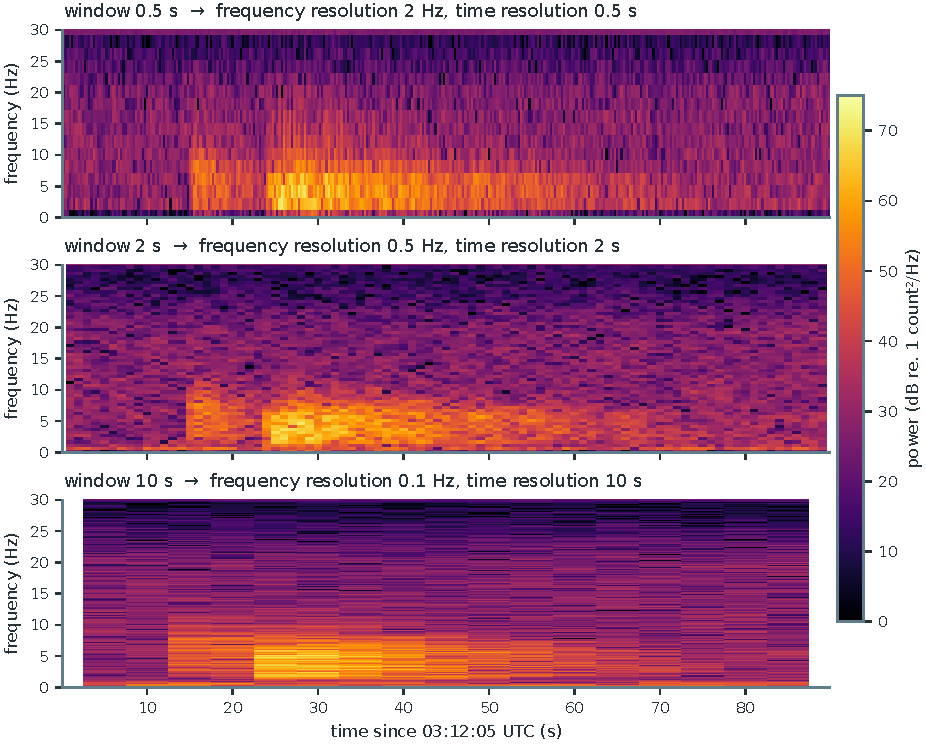
\includegraphics[width=\linewidth]{theory-spectrogram-tradeoff}
\caption{The demo local earthquake (EHZ, 03:12:05--03:13:35 UTC) with three window lengths, computed by the
application's \code{spectrogram}. Short windows localise the P and S onsets in time; long windows resolve
frequency.}\label{fig:tradeoff}
\end{figure}

\section{The window used by RS3D}
The application calls SciPy's \code{spectrogram} without specifying a window, so SciPy's default applies: a periodic
\textbf{Tukey window with $\alpha=0.25$}, which is flat in the middle and tapers with half-cosine edges over 25\,\% of the
window. \Cref{tab:windows} gives its measured properties: it is close to rectangular, with coherent gain $0.875$,
noise bandwidth $1.10$ bins, and a peak sidelobe only $-13.6$~dB below the peak. This is a defensible choice for
\emph{locating} events (the main lobe is narrow and little signal is lost) but it leaks more than the Hann window of the
amplitude spectrum.

\begin{rs3dwarn}[Leakage from strong low-frequency noise]
Because the Tukey window has high sidelobes that decay slowly, a very strong low-frequency signal, such as the
microseism, leaks a little energy into higher bins. For a typical RS3D day the effect is smaller than the dynamic range of the
colour scale, but a spectrogram of data with a large low-frequency component should be read with this in mind. Replacing the
window by a Hann window is a one-line change should it ever be needed.
\end{rs3dwarn}

\section{Choosing the window length: the 360 rule}
No single window length suits both a two-minute detail view and a 24-hour overview. The application chooses it from
the duration $T$ of the selection:
\begin{equation}\label{eq:window}
  T_w = \min\!\bigl(\max(T/360,\;1\ \mathrm{s}),\; 600\ \mathrm{s}\bigr).
\end{equation}
With 50\,\% overlap a record of duration $T$ yields about $2T/T_w-1\approx 719$ columns, a few hundred to a thousand, which
is about what a screen can display and what the browser can plot quickly, whatever the duration. The limits keep the
window between 1~s (so that even a short selection has a usable number of samples) and 10~minutes. \Cref{fig:rule} shows the
resulting window length and frequency resolution; \cref{tab:examples} gives worked examples.

\begin{figure}[tbp]
\centering
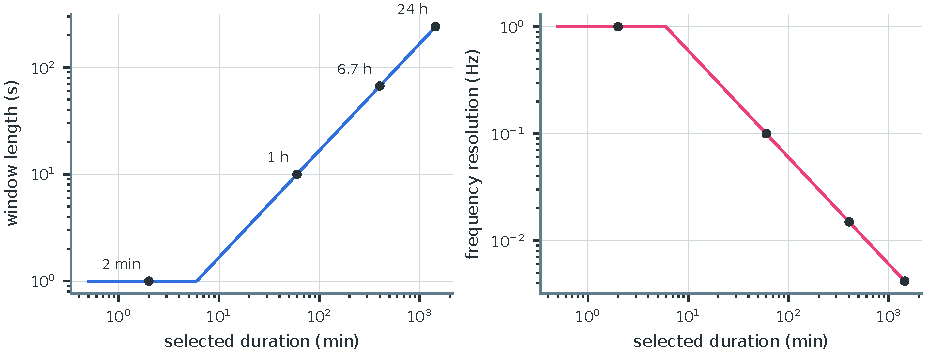
\includegraphics[width=\linewidth]{theory-window-rule}
\caption{The window-length rule~\eqref{eq:window} (left) and the frequency resolution it implies (right) as a function
of the selected duration.}\label{fig:rule}
\end{figure}

\begin{table}[tbp]
\centering\small
\caption{Window length, frequency resolution and number of columns for typical selections.}\label{tab:examples}
\begin{tabular}{@{}lrrr@{}}
\toprule
Selection & $T_w$ (s) & $\df$ (Hz) & columns\\ \midrule
2 minutes (detail view) & 1 & 1.0 & 239\\
1 hour & 10 & 0.1 & 719\\
6.7 hours & 67 & 0.015 & 719\\
24 hours & 240 & 0.004 & 719\\
\bottomrule
\end{tabular}
\end{table}

\section{Gaps}
A window that touches a gap would mix real signal with filler. The application therefore sets the samples of a gap to zero
for the transform and then marks \emph{every column whose window overlaps a gap} as not-a-number, drawn as blank. The
columns on either side of a gap are computed from complete windows only, so a gap does not smear into its
neighbours (\cref{fig:specday}, where two gaps are visible as white bars).

\section{From numbers to pixels}
The application never sends the full grid to the browser. The $(\text{frequency}\times\text{time})$ matrix is
\emph{binned} to at most $400\times200$ cells; each cell shows the mean of the decibel values it covers, and cells with no
valid value are left out. Averaging \emph{decibels} is the same as taking a geometric mean of power, which slightly
underestimates narrow peaks compared with averaging power. The colour scale runs from the 2nd to the 98th percentile of
the displayed values, so that a few extreme cells do not wash out the picture.

\begin{figure}[tbp]
\centering
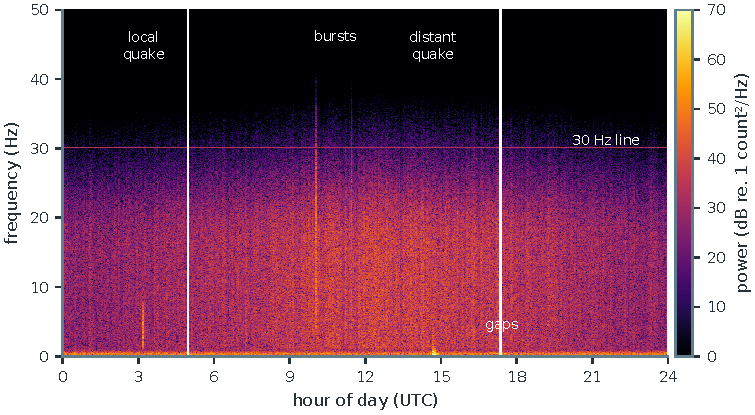
\includegraphics[width=\linewidth]{theory-spectrogram-day}
\caption{A full-day spectrogram of the demo EHZ channel computed with the application's functions (window 240~s). The
day--night change in cultural noise, the local and distant earthquakes, two noise bursts, the 30~Hz instrument line and the
two gaps (white) are all visible.}\label{fig:specday}
\end{figure}

\section{Reading a spectrogram}
\begin{description}[leftmargin=2.2cm,style=nextline]
\item[Earthquake] a vertical streak starting abruptly at the P arrival; energy at higher frequencies arrives first and the
  S wave follows, with a coda fading at lower frequencies.
\item[Man-made burst] a short, broadband streak with no coda; compare the two bursts at about 10--11~h in
  \cref{fig:specday}.
\item[Narrow horizontal line] a persistent single frequency: usually electrical interference or machinery, here the
  30~Hz instrument line.
\item[Slow day--night change] cultural noise, strongest in working hours.
\item[Low-frequency band] the ocean microseism, near 0.1--0.3~Hz.
\end{description}

\begin{rs3dapp}
\code{spectrogram(trace, window\_s, overlap=0.5)} in \file{core/spectro.py} returns window-centre times, frequencies and
decibel values; \code{window\_for(duration)} is Eq.~\eqref{eq:window}. The page code
(\file{app/charts.py}, \code{spectrogram\_options}) performs the binning and colour scaling.
\end{rs3dapp}
